\chapter{Correlation from non-equilibrium Green's functions} 
\label{chaptercorr}
\section{A simple introduction to non-equilibrium Green's functions}
In this section we present a simple introduction to the non-equilibrium Green's functions, following the lines of Ref.~\cite{kremp}. \\
In quantum mechanics a many-body system is characterised by its Hamiltonian, i. e. by:
\be
H=\sum^N_{i=1} \frac{\pp^2_i}{2m} + \sum_{i}^{N} V_{ei} (\rr_i) + \sum_{i<j}^N V_{ee}(\rr_i - \rr_j ), 
\label{fullH}
\ee
where $V_{ei}$ is the potential generated by the ions and $V_{ee}$ is the electron-electron interaction.
This last term in the previous equation makes the many-body problem impossible to solve in the case of three  or more interacting particles. However we can always try to find a solution of the Hamiltonian [Eq.~\ref{fullH}] as a linear combination of the
single-particle solutions of a non-interacting problem, i. e. the solution of the  above Hamiltonian
without the electron-electron interaction. The non-interacting solution constitutes a complete basis set in the form:
\be
| b_1, b_2,...,b_N \rangle = \frac{1}{\sqrt{N!}} a^+(b_1) .... a^{+}(b_N) | 0 \rangle
\ee
where $|0\rangle$ is the state without particles and the creation operators $a^+(b_i)$ create a particle
in a given state $b_i$ of our single particle Hamiltonian. The properties of the creation/destruction
operators guarantee the correct Fermi statistics. Once we have determined the wave-function, or at least,
an approximate wave-function, all the observables can be expressed in terms of  $a$ and $a^+$ operators.\\
Proceeding in this way is a formidable task, because in a solid the number of particles is of the order
of the Avogadro's number $N \simeq 10^{23}$, i.e. practically an infinite number of particles.\\
But we do not need all this information to characterise a physical system. In fact the mean value of any
single particle operator as dipole, momentum, etc.. can be expressed in terms of the single particle density matrix, without the need of the full wave-functions:
\bea
\gamma (\xx_1,\xx_1') &=& N \int d \xx_2 d \xx_3... d \xx_N \Psi (\xx_1,\xx_2,...,\xx_N) \Psi^* (\xx_1,\xx_2,...,\xx_N)\\
\langle  A \rangle &=& tr \left ( \gamma  A \right ),
\eea
where $A$ is a single particle operator, and $\gamma (\xx_1,\xx_1')$ the one-body density matrix.
Obviously the mean-value of a s-particle operator may be evaluated by means of the s-particle density matrix. \\ If we know the EOMs for the density matrix it will be possible to
follow the full many-body dynamics without passing by the full wave-function.\\
Based on this idea John Von Neumann in 1927 derived an equation for the temporal evolution of the density matrix operator\cite{neumann}:
\be
i \frac{\partial \gamma}{\partial t} = [\HH, \gamma].
\label{densmat}
\ee
This equation can be obtained from the  Schr\"odinger equation, and provides an equivalent description of quantum mechanics. The major problem of Eq.~\ref{densmat} is that it is not a closed equation. If we write down explicitly [Eq.~\ref{densmat}] for the single particle density matrix we immediately realise that the r.h.s. depends from the two-body density matrix, whose EOMs will depend from the three-body density matrix and so on. This set of equations, called the BBGKY hierarchy (Bogoliubov-Born-Green-Kirkwood-Yvon hierarchy), describes the full  dynamics of a system with a large number of interacting particles.\cite{bonitz} \\
The solution of the BBGKY hierarchy has the same complexity of the initial  Schr\"odinger equation. 
For this reason different scientists searched for a closed form of Eq.~\ref{densmat} that involves only a limited order of density matrices. The simplest decoupling of the hierarchy is achieved by the application of the Hartree-Fock (HF) approximation:
\be
\gamma (\rr_1,\rr_2,\rr_1',\rr_2') =  \gamma (\rr_1,\rr_1') \gamma (\rr_2,\rr_2') -  \gamma (\rr_1,\rr_2') \gamma (\rr_2,\rr_1').
\ee
In the HF the two-particle density matrix is expressed in terms of the single particle one, and therefore the EOMs for single-particle density matrix are closed. Clearly HF is not a satisfying approximation to describe electronic properties of real-systems. In the literature many different ways to close the BBGKY equations have been proposed that are able to treat correlations at different levels (for a discussion see Ref.~\cite{bonitz,RevModPhys.74.895} and references there in).\\
The density matrix formalism is a very powerful tool to study the many-body problems in a large spectra of situations, however it presents two important limitations that motivated the development of Green's function theory. First of all, there are  different situations where we are interested in time-dependent (or frequency dependent) correlation functions that are not directly accessible from the density matrix. Second the decoupling of the BBGKY hierarchy equations is not an easy task, especially in systems with many particles as for instance bulk materials. Now we will see how it is possible to generalise the density matrix approach to solve these two issues. \\
If we write the density matrices in term of field operators:
\be
\gamma (\rr_1 ... \rr_s,\rr_1'... \rr_s) = \langle \psi^\dagger(\rr_1',t) ... \psi^\dagger(\rr_s',t) \psi(\rr_1,t) ... \psi(\rr_s,t)  \rangle,
\ee
it follows that Green's functions are a generalisation of s-particle density matrices with field operators at different times:
\be
G^<(\rr_1,t_1 ... \rr_s,t_s,\rr_1',t_s' ... \rr_s, t_s') = \left(-\frac{1}{i} \right)^s \langle \psi^\dagger(\rr_1',t_1') ... \psi^\dagger(\rr_s',t_s') \psi(\rr_1,t_1) ... \psi(\rr_s,t_s)  \rangle.
\ee
Different arrangements of the field operators correspond to different time-correlation functions, i.e. different Green's functions: greater, casual, retard or advanced.
As in the case of density matrices the properties of a full many-particle systems can be described in terms of Green's functions. But differently from density matrices we have a direct access to dynamical properties, as for instance response functions, excitation energies and so on (see Chapter 3 of Ref.~\cite{kremp}).\\
A central task of the theory is the determination of these functions. The dynamics of the Green's functions can be derived from the EOMs of the field operators. For example for the $G^<$ we obtain:
\be
\left( i \frac{\partial}{\partial t_1} + \frac{\nabla_i^2}{2m} - U(1) \right) G^<(1,1') - i \int d2 V(1,2) G^<(12,1'2^+) = 0
\ee
where $1,2$ are indexes for both time and position, the $2^+$ is the limit of $2' \rightarrow 2$ with $t_2'> t_2$, and $U(1)$ is the external potential.
As in the case of reduced density matrix, the EOMs for the single particle Green's functions are not closed and depend from two particle Green's functions and so on. The problem may, in principle, be solved using equations similar to the BBGKY hierarchy, the so called Martin-Schwinger hierarchy equations. However Green's function presents a major advantage that is the possibility to construct a single particle operator, the self-energy $\Sigma$, that is not local in time and space and allows us to close the EOMs in the form:
\be
\int_C d \bar 1 \left [ G_0^{-1} (1 \bar 1) - U(1\bar1) - \Sigma (1 \bar 1) \right ] G(\bar 1 1)  = \delta(1- 1'),
\label{kbeq}
\ee
where $G_0$ is the independent particle Green's function and the integral is performed on the Keldysh contour.\footnote{In this introduction we have no space to derive and explain Eq.~\ref{kbeq}, for more details see the textbooks \cite{kremp,schafer,kadanoff,haug2008quantum}.}\\
This famous equation was derived for the first time by Kadanoff and Baym and by Keldysh. It is a generalisation of the Dyson equation from the field theory to quantum statistics. Equation~\ref{kbeq} describes time evolution of real-time Green's functions under equilibrium and non-equilibrium conditions. \\
Of course, all problems of the hierarchy equations are now transferred to the self-energy construction.
In the literature different approaches have been proposed to construct self-energies. In this chapter we will use the so-called GW approximation. The GW self-energy is the first order correction, in term of screened Coulomb interaction, obtained from many-body perturbation theory\cite{aryasetiawan1998gw}. This approximation has been derived by Hedin\cite{hedin1999correlation} for the electron gas and then applied to semiconductors by Hanke, Sham and Strinati\cite{PhysRevB.25.2867}.\footnote{As it is often the case in  physics, the GW self-energy originates from previous studies on the electron gas, based on perturbation theory in terms of screened Coulomb interaction performed by DuBois, Kadanoff, Baym and Bonch-Bruevich and Tyablikov.} The GW corrections have shown a  clear  improvement for band gaps\cite{aryasetiawan1998gw,Aulbur19991}, level ordering\cite{faber2011first} and gradients of the electronic levels respect to the atomic displacements\cite{faber2015exploring}, when compared to available experimental data.\\
In the next sections, starting from a non-equilibrium formulation of the GW self-energy\cite{PhysRevB.69.205204}, we will derive an effective single-particle Hamiltonian for our real-time dynamics. 

\section{General Introduction}
%%%%%%%%%%%%%%%%%%%%%%%%%%%%%%%%%%%%%%%%%%%%%%%%%%%%%%%%%%%%%%%

Real-time methods have proven their utility in calculating optical properties of finite systems mainly within time-dependent density functional
theory (TDDFT).\cite{PhysRevB.62.7998,PSSB:PSSB200642067,sun:234107} On the other hand extended systems have been mostly studied by using many-body  perturbation
theory (MBPT) within the linear response regime~\cite{strinati}. 
The different treatment of correlation and nonlinear effects marks the range of applicability of the two approaches. The real-time TDDFT makes
possible to investigate nonlinear effects like second harmonic generation\cite{takimoto:154114} or hyperpolarizabilities of 
molecular systems\cite{PSSB:PSSB200642067}.
However, as we will see in Chapter~\ref{chaptertddft} TD-DFT is not a correct theory to describe excitations at zero momentum $\qq=0$ in extended systems.
For this reason, even with the exact exchange correlation functional TD-DFT is not suppose to reproduce the exact response functions in solids.
On the contrary MBPT allows to include correlation effects using controllable and systematic approximations for the self-energy $\Sigma$,
that is a one-particle operator non-local in space and time.
$\Sigma$ can be evaluated within different approximations, among which one of the most successful is the so-called GW
approximation\cite{Aulbur19991}.
Since its first application to semiconductors\cite{PhysRevLett.45.290} the GW self-energy has been shown to
correctly reproduce quasi-particle energies and lifetimes for a wide range of materials\cite{Aulbur19991,faber2013many}.
Furthermore, by using the static limit of the GW self-energy as scattering potential of the
Bethe-Salpeter equation (BSE)\cite{strinati}, it is possible to calculate response functions including electron-hole interaction
effects.

In recent years, the MBPT approach has been merged with density-functional theory (DFT) by using the Kohn-Sham Hamiltonian as zeroth-order term in the
perturbative expansion of the interacting Green's functions. This approach is parameter free and completely \emph{ab-initio}~\cite{Onida}.  
However MBPT is a very cumbersome technique that, based on a perturbative concept, increases its level of complexity with
the order of the expansion. As an example, this makes the extension of this approach beyond the linear response regime quite complex, though there have been recently some applications in nonlinear optics.~\cite{Chang2002,Leitsmann2005,PhysRevB.82.235201}
A generalisation of MBPT to non-equilibrium situations has been proposed by Kadanoff and Baym and Keldysh\cite{kadanoffbaym}. 
In their seminal works the authors derived a set of equations for the real-time Green's functions, the Kadanoff-Baym equations (KBE's), that provide the basic tools of the non-equilibrium Green's Function theory and allow essential advances in non equilibrium statistical mechanics\cite{kadanoffbaym}.   
Both the standard MBPT and non-equilibrium Green's Function theory are based on
the Green's function concept. This function describes the time propagation of a single particle excitation under the action of an external perturbation.  
In the equilibrium MBPT, due to the time translation invariance,
the relevant variable used to calculate the Green's functions is the frequency $\omega$. Instead, out of equilibrium, in all non steady-state situations, the time variables acquire a special role and much more attention is devoted to the their propagation properties. 
The time propagation avoids the explosive dependence, beyond the linear response, of the MBPT on high order Green's functions. Moreover the KBE are
non-perturbative in the external field therefore weak and strong fields can be treated on the same footing. 

One of the first attempts to apply the KBE's for investigating optical properties of semiconductors was presented in the seminal paper of Schmitt-Rink and co-workers.~\cite{PhysRevB.37.941} 
Later the KBE's were applied to study quantum wells,~\cite{PhysRevB.58.2064} laser excited
semiconductors,~\cite{PhysRevB.38.9759} and luminescence~\cite{PhysRevLett.86.2451}. However, only recently it was possible to simulate the Kadanoff-Baym
dynamics in real-time.~\cite{Kohler1999123,PhysRevLett.103.176404,PhysRevLett.84.1768,PhysRevLett.98.153004} 
In this chapter we combine a simplified version of the KBE's with DFT in such a way to obtain a parameter-free theory that is able to reproduce and predict
ultra-fast and nonlinear phenomena in crystalline solids and nano-structures 
(Sec.~\ref{tdbse_section}). This approach, that we
will address as time-dependent BSE, reduces to the standard BSE for weak perturbations (Sec.~\ref{linear_response}) but, at the same time when coupled
with Modern Theory of Polarisation (see Chapter~\ref{chapterberry}), naturally describes optical excitations beyond the linear regime. 
After discussing some relevant aspects of the practical implementation of our approach (Sec.~\ref{teospectro}), we 
exemplify how it works in practice by calculating the optical absorption spectra of {\it h}-BN, and we'll apply it to the 
second harmonic generation in monolayer {\it h}-BN and MoS$_2$.

\section{The time-dependent Bethe-Salpeter equation}
%%%%%%%%%%%%%%%%%%%%%%%%%%%%%%%%%%%%%%%%%%%%%%%%%%%%%%%%%%%%%%%
\label{tdbse_section}                                        
We derive here a novel approach to solve the time evolution of an electronic
system with Hamiltonian coupled with an external field,
\be
\label{hamiltonian}
\hat{H} = \hat{h} + \hat{H}_{mb} + \hat{U},     
\ee
where $U$ represents the electron-light interactions (see
Sec.~\ref{ss:solution} for its specific form). As usually done in MBPT, $\hat{H}$
is partitioned in an (effective) one-particle Hamiltonian
$\hat h$ and a part containing the many-particle effects $\hat{H}_{mb}$. 

In our derivation, we take as starting point the KBE's that we briefly introduce in
Sec.~\ref{ss:KBEs} (see e.g. Refs.~\cite{kremp} for a systematic
treatment). Then, in Sec.~\ref{ss:KS-CHSX} we proceed in analogy with
the equilibrium MBPT: first, we define $\hat h$ as the Hamiltonian of the Kohn-Sham
system, second we introduce the same approximations for the
self-energy operator. As a result we obtain the analogous of the
successful $GW$+BSE approach for the non-equilibrium case. Indeed in
Sec.~\ref{linear_response} we show that our approach, the
time-dependent BSE, reduce to the $GW$+BSE in the linear regime.\footnote{Notice that a real-time version
        of the Bethe-Salpeter equation was already proposed in Ref.~\cite{PhysRevB.67.085307} as
an efficient method to solve the BSE, but it was limited to the linear response.}

\subsection{The Kadanoff-Baym equations}
%%%%%%%%%%%%%%%%%%%%%%%%%%%%%%%%%%%%%%%%%%%%%%%%%%%%%%%%%%%%%%%
\label{ss:KBEs}
Within the KBE's, the time evolution of an electronic system 
coupled with an external field is described by the equation of motion for the non-equilibrium Green's functions $G\(\rr,t;\rr' t'\)$ ~\cite{kadanoffbaym,kremp,schafer}.  
To keep the formulation as simple as possible and, being interested
only in long wavelength perturbations,
we expand the generic $G$ in the eigenstates $\{\varphi_{n,\kk}\}$ of the $\hat{h}$ Hamiltonian for a fixed momentum point $\kk$:
\be
\label{GFdefinition}
\[\GG_{\kk}\(t_1,t_2\)\]_{n_1 n_2}\equiv G_{n_1 n_2, \kk }(t_1,t_2)=\int
\varphi^*_{ n_1\kk}({\mathbf r}_1) G\(\rr_1,t_1;\rr_2,t_2\) \varphi_{n_2\kk}({\mathbf
r}_2){\mathrm d}^3r_1{\mathrm d}^3r_2.
\ee
As the external field does not break the spatial invariance of the system $\kk$ is conserved.
Notice that both the Green's functions and the self-energies will depends from two times $t_1, t_2$ because we are in an out-equilibrium situation. These two times can be also rewritten in terms of $t = (t_1 + t_2)/2$ and $\tau = t_1 - t_2$, where $t$ is the physical time and $\tau$ a fictitious time related to quantum correlations.\\
Within a second-quantization formulation of the many-body problem, the equation of motion for the Green's function described by Eq.~\eqref{GFdefinition} are obtained
from those for the creation and destruction operators.  However the resulting equations of motion for $\GG_{\kk}$ are not closed:
they depend on the equations of the two-particle Green's function that in turns depends on the three-particle Green's function and so on.
In order to truncate this hierarchy of equations, one introduces the self-energy operator $\SiS_{\kk}(t_1,t_2)$, a non-local and frequency dependent
one-particle operator that holds information of all higher order Green's functions. 
A further complication arises with respect to the equilibrium case because of the lack of time-translation invariance in non-equilibrium phenomena that implies that 
$\SiS_{\kk}(t_1,t_2)$ and $\GG_{\kk}(t_1,t_2)$ depend explicitly on both $t_1,t_2$. Then, one can define an
advanced $\SiS_{\kk}^a$ ($\GG_{\kk}^{\mathrm a}$), a retarded $\SiS_{\kk}^r$ ($\GG_{\kk}^{\rr}$), a greater and a lesser $\SiS_{\kk}^>,\SiS_{\kk}^<$ ($\GG_{\kk}^>,\GG_{\kk}^<$) self-energy
operators (Green's functions) depending on the ordering of $t_1,t_2$ on the time axis. 
Finally, 
%by using the concept of self-energy 
the following EOM for the $\GG_{\kk}^<$ is obtained (see e.g. Ch.~2 of
Ref.~\cite{kremp} for more details):
\begin{multline}
 i\hbar  \frac{\partial}{\partial t_1} G^<_{n_1n_2\kk}(t_1,t_2)=\mbox{}  \delta(t_1-t_2)\delta_{n_1n_2}    \\
+  h_{n_1n_1\kk}(t_1) G^<_{n_1n_2\kk}(t_1,t_2) + \sum_{n_3}U_{n_1n_3\kk}(t_1) G^<_{n_3n_2\kk}(t_1,t_2) \\
+  \sum_{n_3} \int \mathrm{d}t_3 \big( \Sigma^{\rr}_{n_1n_3\kk}(t_1,t_3)G^<_{n_3n_2\kk }(t_3,t_2) 
+ \Sigma^<_{n_1n_3\kk}(t_1,t_3) G^{\mathrm a}_{n_3n_2\kk}(t_3,t_2)\big) .
\label{eqmotGone}
\end{multline}
This equation, together with the adjoint one for $ i\hbar  \frac{\partial}{\partial t_2} G^<$, describes the
evolution of the lesser Green's function $\GG_{\kk}^<$ that gives
access to the electron distribution ($\GG_{\kk}^<(t,t)$) and to the
average of any one-particle operator such as for example the electron
density [Eq.~\eqref{eqden}], the linear polarisation and the current.  However, in general $\Sigma^{\rr},\Sigma^<$ and  $\GG_{\kk}^{\mathrm a}$ depend on $\GG_{\kk}^>$, so that in addition to Eq.~\eqref{eqmotGone} the corresponding equation for the $\GG_{\kk}^>$ has to be solved. 

Then, in principle, to determine the non-equilibrium Green's function in presence of an external perturbation one needs  to solve the system of coupled equations for $\GG_{\kk}^>,\GG_{\kk}^<$, known as KBE's. Indeed, this system has been implemented within several approximations for the self-energy in model
systems\cite{Kohler1999123,PhysRevLett.103.176404}, in the homogeneous electron gas\cite{PhysRevLett.84.1768}, and in atoms\cite{PhysRevLett.98.153004}.
The possibility of a direct propagation in time of the KBE's provided, in these systems, valuable insights on the real-time dynamics of the electronic excitations, as their lifetime and transient effects.\cite{Kohler1999123,PhysRevLett.103.176404,PhysRevLett.84.1768,PhysRevLett.98.153004} 
Nevertheless, the enormous computational load connected to the large number of degrees of freedom {\it de facto} prevented the application of this method to crystalline solids, large molecules and nano-structures. In the next subsection we show a simplified approach---grounded on the DFT---that while capturing most of the physical effects we are interest in, makes calculation of ``real-world'' systems feasible. 

\subsection{The Kohn-Sham Hamiltonian and an approximation for the self-energy}
%%%%%%%%%%%%%%%%%%%%%%%%%%%%%%%%%%%%%%%%%%%%%%%%%%%%%%%%%%%%%%%
\label{ss:KS-CHSX}

In analogy to MBPT for the equilibrium case,
we choose as $\hat{h}$ in Eq.~\eqref{hamiltonian} the Kohn-Sham Hamiltonian,~\cite{PhysRev.140.A1133} 
\be
\hat{h} = -\frac{\hbar^2}{2m} \sum_i \nabla_i^2 + 
\hat{V}_{eI} + \hat{V}^H[\tilde \rho]   + \hat{V}^{xc}[\tilde \rho], \label{eq:kshamH}
\ee
where $\hat{V}_{eI}$ is the electron-ion interaction, 
%with the ions
%usually described by norm-conserving
%pseudopotentials,\cite{troullier}
$\hat{V}^H$ is the Hartree potential and
$\hat{V}^{xc}$ the exchange-correlation potential.
Within DFT, the Kohn-Sham Hamiltonian corresponds to the independent particle system
that reproduces the ground-state electronic density $\tilde \rho$ of
the full interacting system ($\hat h + \hat H_{\text{mb}}$), that is
\be
\tilde \rho = \sum_{n\kk} f_{n\kk}|\varphi(\rr)|^2,
\label{eq:KSden}
\ee
where $f_{n\kk}$ is the Kohn-Sham Fermi distribution. 

The EOM for the $\GG_{\kk}^<$  [Eq.~\eqref{eqmotGone}] can be greatly simplified by choosing 
a static approximation for the self-energy,
\begin{subequations}
\begin{align}
{\bf\Sigma}^{\rr} (t_1,t_2) & = \left[ {\bf\Sigma}^{\mathrm {cohsex}} (t_1) - {\bf V}_{xc} \right ] \delta(t_1 - t_2) \label{eq:appcsx}\\
{\bf\Sigma}^<(t_1,t_2) & =0 \label{eq:appret}
\end{align}
\end{subequations}
where the usual choice is ${\bf\Sigma}^{\mathrm {cohsex}}$, the so-called Coulomb-hole plus screened-exchange self-energy (COHSEX)\cite{PhysRevB.38.7530}. In Eq.~\ref{eq:appcsx} we subtracted the correlation effects already accounted by Kohn-Sham Hamiltonian $\hat{h}$.
The COHSEX is composed of two parts:
\bea
\Sigma^{\text{sex}}(\mathbf r,\mathbf r',t)=i W(\mathbf r,\mathbf r'; G^<)G^<(\mathbf r,\mathbf r',t), \\
\Sigma^{\text{coh}}(\mathbf r,\mathbf r',t)= -W(\mathbf r,\mathbf r'; G^<) \frac{1}{2}\delta(\mathbf r-\mathbf r'),
\label{coh_anx_sex}
\eea
where $W(\mathbf r,\mathbf{r'}; G^<)$ is the Coulomb interaction in
the random-phase approximation (RPA) and $G^<(\rr,\rr',t)$ is the time-diagonal lesser Green's function $G^<(\rr,\rr',t)=G^<(\rr,\rr',t,t)$. These two terms are obtained as a
static limit of the $GW$ self-energy (see Ch.4 of Ref.~\cite{kremp} and
Refs.~\cite{PhysRevB.38.7530, PhysRevB.69.205204}). 

If we insert the approximated self-energy Eqs.~\eqref{eq:appcsx}--\eqref{eq:appret} in Eq.~\eqref{eqmotGone}, the EOM for the $\GG_{\kk}^<$  does not depend anymore on ${\bf G}^>$.
Moreover, since the COHSEX self-energy is local in time, and depends only on $G^<(\rr,\rr',t)$, Eq.\eqref{eqmotGone} can be combined with the adjoint one for $\frac{\partial}{\partial t_2} G^<_{n_1n_2\kk}(t_1,t_2)$ in such a way to have a closed equation in $t=(t_1+t_2)/2$:

% (see Refs.~\cite{kremp,schafer} for a detailed discussion):
\begin{multline}
\label{eqmotGcohsex}
 i\hbar  \frac{\partial}{\partial t} G_{n_1,n_2,\kk}^<(t)=
 \left [ \hh_{\kk} + \UU_{\kk}(t) +  \VV_{\kk}^H[\rho] -
   \VV_{\kk}^H[\tilde \rho] \right .\\
   \left . + (\SiS_{\kk}^{\mathrm{cohsex}} (t)
   -\VV_{\kk}^{xc}[\tilde \rho]), \GG_{\kk}^<(t)\right ]_{n_1,n_2}.
\end{multline}
where the term $\VV_{\kk}^H[\rho] - \VV_{\kk}^H[\tilde \rho]$ is the induced variation of the Hartree term that generates the exchange in the BSE, and $\rho$ is the density obtained from the $G^<$ as 
\be
\label{eqden}
\rho(\mathbf r,t) = \frac{i}{\hbar} \sum_{n_1n_2\kk} \varphi_{n_1 \kk} (\mathbf r)  \varphi^*_{n_2 \kk}  (\mathbf r) G^<_{n_2n_1\kk}(t).
\ee
After reducing to a single time, \eqref{eqmotGcohsex} is equivalent to a density matrix approach with a potential local in time. 
%However, even if the equations of motion in Eq.~\ref{eqmotGcohsex}
%considerably simplify the dynamics with respect to the KBE's, they neglect dynamical effects. Indeed the COHSEX approximation is known to induce a too 
%large renormalization of the one-particle eigenvalues. Some of these effects can be partially
%reintroduced by using the so-called Generalized Kadanoff-Baym ansatz\cite{GKBA}, that we plan to investigate in a forthcoming paper.
%
However, despite the full real-time COHSEX dynamics [Eq.~\ref{eqmotGcohsex}] is an appealing
option considerably simplifying the dynamics with respect to the KBE's,
it neglects the dynamical dependence of the self--energy operator. This, in practice, induces a consistent renormalization 
of the quasi-particle charge\cite{PhysRevLett.45.290} in addition to an opposite enhancement of the optical properties.~\cite{PhysRevLett.91.176402}
In the COHSEX approximation both effects are neglected.
%, that is a quite crude
%approximation. Indeed, it is known that dynamical effects 
%on the quasi-particle properties\cite{PhysRevLett.45.290} are
%extremely important, and COHSEX largely overestimates the
%renormalization factors. 
At the level of response properties for
most of the extended systems dynamical effects are either negligible or very small\footnote{
Recently it has been shown that dynamical effects in the BSE can be important for finite
systems, see Refs.~\cite{bsedynamic,PhysRevB.77.115118}} and it has been shown that they  
partially cancel with the  quasi-particle renormalization factors.~\cite{PhysRevLett.91.176402} 

Therefore we modify Eq.~\ref{eqmotGcohsex} in order to include only the effect
of the dynamical self-energy on the renormalization of the quasi-particle energies, that is the most
important effect.
Also in this case, our idea is to proceed in strict analogy with equilibrium MBPT and to derive a real-time equation that reproduces the fruitful combination of the $G_0W_0$
approximation---for the one-particle Green's function---and of the BSE with
a static self-energy---for the two-particle Green's function. 
Indeed the $G_0W_0$+BSE is the state-of-the-art approach to study optical
properties within MBPT.~\cite{Onida} 
To this purpose Eq.~\eqref{coh_anx_sex} is modified as:
\begin{multline}
\label{tdbse}
 i \hbar  \frac{\partial}{\partial t} G^<_{n_1n_2\kk}(t)= 
\left [ \hh_{\kk} + \Delta \hh_{\kk} + \UU_{\kk} +\VV_{\kk}^H[\rho] - \VV_{\kk}^H[\tilde \rho] \right . \\
 \left . + \SiS_{\kk}^{\text {cohsex}}[G^<] - \SiS_{\kk}^{\text{cohsex}}[\tilde G^<], \GG_{\kk}^<\(t\) \right ]_{n_1n_2}. 
\end{multline}
$\Delta \hh$ is a scissor operator\cite{Onida} that
applies the $G_0 W_0$ correction to the Kohn-Sham eigenvalues, $e_{n_1\kk}^{KS}$,
\be
\label{eq:sciss}
\[\Delta \hh_{\kk}\]_{n_1,n_2} =  \left ( e_{n_1\kk}^{G_0W_0}  -e_{n_1\kk}^{KS}  \right ) \delta_{n_1,n_2},
\ee
and $\tilde G^<_{n n'}$ is the solution of Eq.~(\ref{tdbse}) for the
unperturbed system ($U=0$)
\be
\tilde G^<_{n n' \kk} = i \hbar f_{n\kk} \delta_{n n'}, \label{gtilde}
\ee
where we assume that the Kohn-Sham Fermi distribution is not changed by the
scissor operator. Note further that in Eq.~\ref{tdbse}, $V^{xc}[\tilde \rho]$ cancels out because it is independent of $G^<(t)$.

Equation~\eqref{tdbse} is the key result of this work. It is equivalent to assume that the
quasi-particle corrections modify only the single particle eigenvalues
leaving unchanged the Kohn-Sham wave functions.  Within equilibrium MBPT this approximation
is very successful for a wide range of materials characterised by weak correlations (see e.g. Refs.~\cite{Onida,Aulbur19991}).\\
Equation~\eqref{tdbse} can rewritten in term of density matrix as:
\bea
i \hbar  \frac{\partial}{\partial t} \gamma_{n_1n_2\kk}(t) &=& \left [ \HH_{mb}(t),\gamma(t) \right ]_{n_1n_2\kk} \\
\HH_{mb} (t) &=& \hh_{\kk} + \Delta \hh_{\kk} + \UU_{\kk} +\VV_{\kk}^H[\rho-\rho_0]+ \SiS_{\kk}^{\text {cohsex}}[\gamma-\gamma_0]. 
\label{mbhamiltonian}
\eea
where $\rho_0$ and $\gamma_0$ are the density and the single particle density matrix at equilibrium. Eq.~\ref{mbhamiltonian}  is the Hamiltonian we will use
in combination with dynamical Berry phase to study the non-linear response in low dimensional systems (see Sec.~\ref{ss:solution}).

%In the next subsection we show that in the linear response limit, the
%time-dependent BSE reduces indeed to the $G_0W_0$+BSE approach within equilibrium
%{\it Ai}-MBPT. 

%\begin{wrapfigure}{r}{0.5\textwidth}
%\begin{center}
%        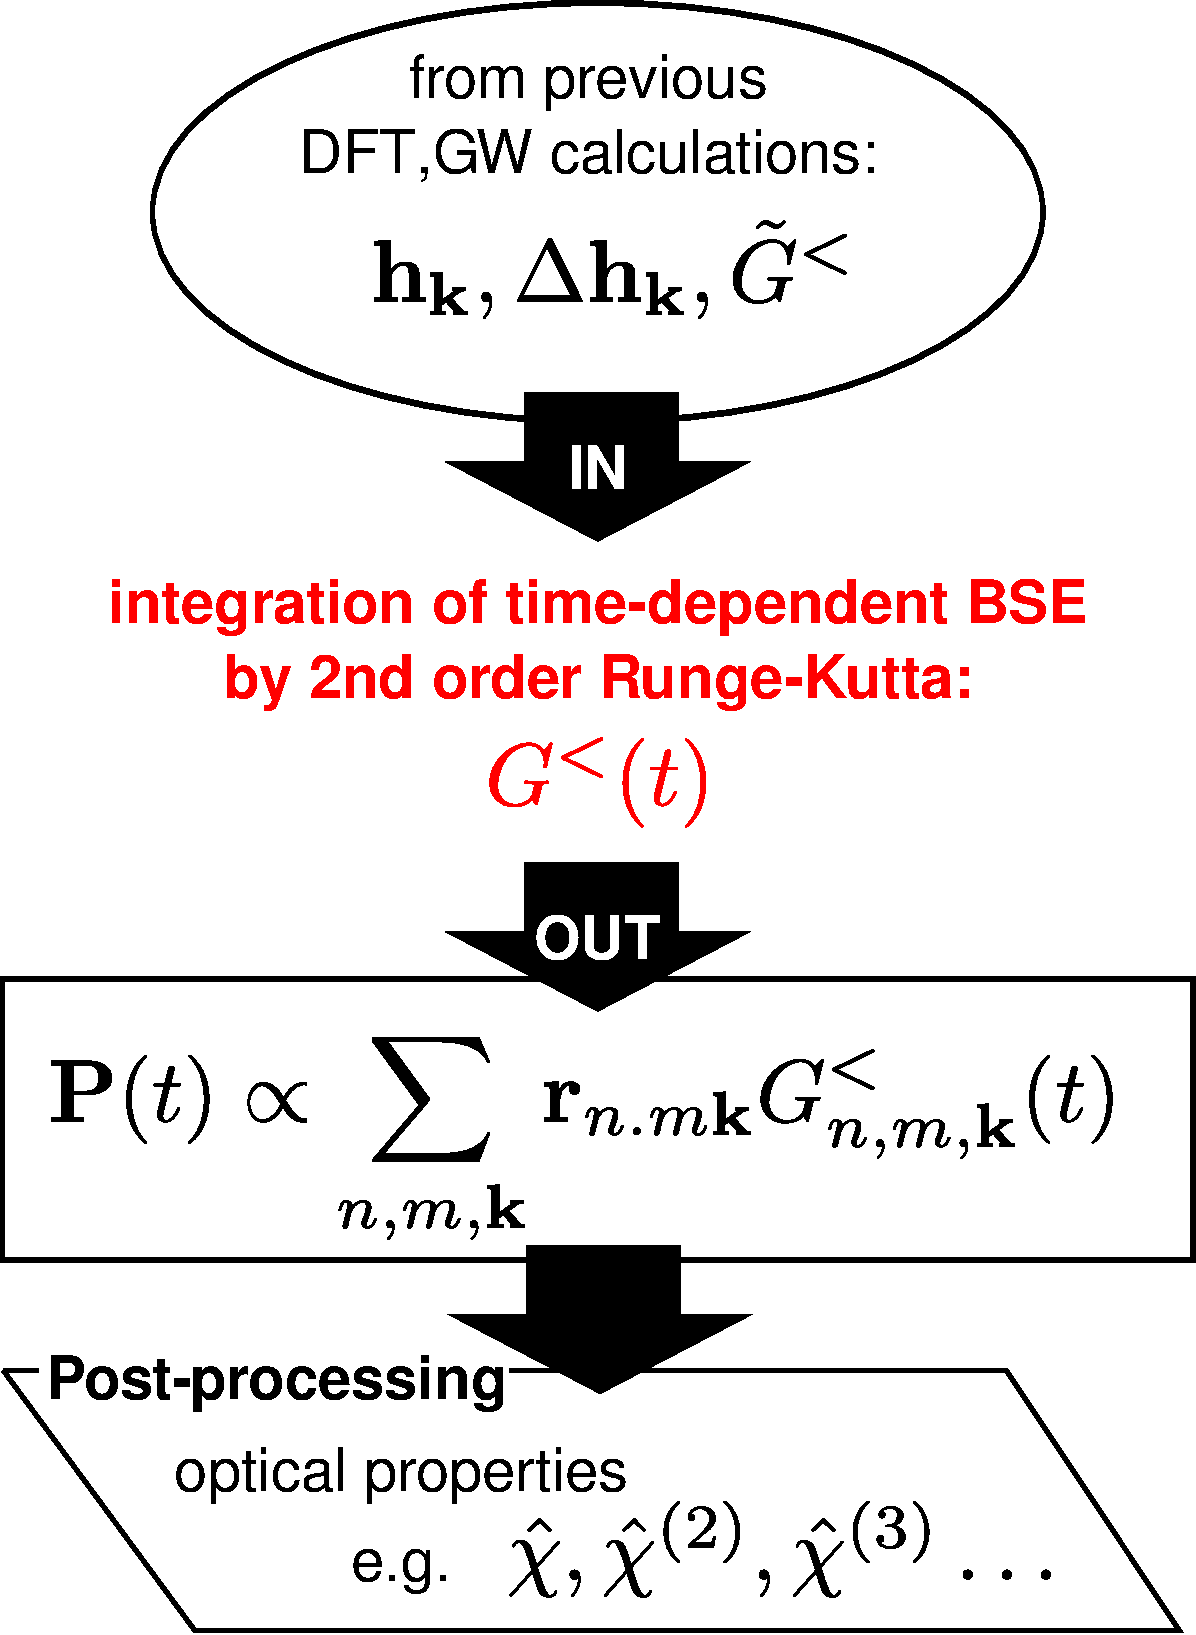
\includegraphics[width=0.4\textwidth]{Figures/scheme-tdbse}
%\caption{\footnotesize{
%Schematic flow of a time-Dependent BSE simulation. See
%Sec.~\ref{ss:solution} for details.}} \label{fg:scheme}
%\end{center}
%\end{wrapfigure}

\subsection{The linear response limit}
% of the time-dependent BSE}
%%%%%%%%%%%%%%%%%%%%%%%%%%%%%%%%%%%%%%%%%%%%%%%%%%%%%%%%%%%%%%%
\label{linear_response}

When an external perturbation $U(t)$ is switched on in Eq.~\eqref{tdbse}, it induces a variation of the Green's function, 
$\Delta \GG_{\kk}^<(t) = \GG_{\kk}^<(t) -  \tilde{\GG}_{\kk}^<$.
In turns, this variation induces a change in the 
self-energy and in the Hartree potential.
In the case of a strong applied laser field these changes depend on
all possible orders in the external field. However for weak fields the
linear term is dominant. 
In this regime it is possible to show analytically that Eq.~\eqref{tdbse}  reduces to the $G_0W_0$+BSE approach\cite{strinati,Aulbur19991}.
Proceeding similarly to Ref.~\cite{bsedynamic} we consider the retarded density-density correlation function:
\be
\label{chi-rr}
\chi^{\mathrm{r}}(\rr,t;\rr',t') =
-i\[\langle \rho(\rr,t)\rho(\rr',t')\rangle 
- \langle \rho(\rr,t)\rangle \langle \rho(\rr',t')\rangle\]\theta\(t-t'\).
\ee
$\chi^{\mathrm{r}}$ describes the linear response of the system to a weak
perturbation, represented in Eq.~\eqref{hamiltonian}  by $U$,
\be
\label{eq:phychi}
\chi^{\mathrm{r}}(\rr,t;\rr',t') = \left. \frac{\langle
  \delta\rho(\rr t) \rangle}{\delta U(\rr^\prime t^{\prime})}\right\vert_{U=0}.
\ee
We start by expanding  $\chi (\mathrm{r})$ in terms of the Kohn-Sham orbitals:
\be
\label{basisChi}
\chi^{\mathrm r}(\rr,t; \mathbf{r'},t'; \mathbf q) =
  \sum_{\substack{i,j,\kk \\ l,m,\kk^\prime} } \chi^{\mathrm r}_{\substack{i,j,\kk \\ l,m,\kk^\prime} }(t,t^\prime; \mathbf q)
\times \varphi_{i,\kk} (\rr)\varphi^*_{j, \mathbf {k+q}} (\rr) \varphi^*_{l, \mathbf {k^\prime}} (\rr')
\varphi_{m, \mathbf {k^\prime+q}} (\rr'),
\ee
where $\qq$ is the momentum, and we define the matrix elements of $\chi^{\mathrm r}$ as,
\be
\label{eq:chimat}
 \chi^{\mathrm r}_{\substack{ij,\kk \\ lm,\kk^\prime} }(t,t^\prime; \mathbf q) =
\iint \mathbf{d}^3r \mathbf{d}^3r^\prime \varphi^*_{i,\kk}(\rr)
\varphi^*_{m, \kk^\prime+\qq} (\rr^\prime)
\varphi_{j,\kk+\qq} (\rr) \varphi_{l, \kk^\prime} (\rr^\prime).
\ee
Since we are interested only in the optical response, in what follows
we restrict ourselves to the case $\qq =0$ and drop the $\qq$
dependence of $\chi^{\mathrm r}$ (for the extension to finite momentum
transfer see Ref.~\cite{PhysRevLett.84.1768}). 
Inserting the expansion for $\chi$ [Eq.~\eqref{basisChi}], $\rho$ [Eq.~\eqref{eqden}] and $U$ ($U_{m,n \kk}\equiv \langle m \kk | U | n \kk \rangle$) in Eq.~\eqref{eq:phychi} we obtain the following relation linking the matrix elements of $\chi^{\mathrm r}$ to the matrix elements of $G^<$:
\be
\label{DDcorFun_n}
\chi^{\mathrm r}_{\substack{ij,\kk \\ lm, \pp }}(t,t^\prime) =
\left. \frac{\delta\langle i G^<_{ji,\kk}(t)\rangle}{\delta U_{lm,\pp}(t^{\prime}
  )}\right\vert_{U=0}.
\ee
Then, we can obtain the equation of motion  for the matrix elements of $\chi^{\mathrm r}$
by taking the functional derivative of Eq.~\eqref{tdbse} with respect to $U_{l,m,\kk}\(t\)$,
\begin{multline}
\label{dtGtt}
-i\hbar \frac{\partial}{\partial t} \chi^{\mathrm r}_{\substack{ij, \kk \\ lm,\pp }}(t,t^\prime)= 
\frac{\delta}{ \delta U_{lm, \pp}(t^{\prime})} [\hh_{\kk} + \Delta \hh_{\kk} + \UU_{\kk}(t) +  \VV_{\kk}^H[\rho(t)] -\VV_{\kk}^H[\tilde \rho]  \\
+  \SiS_{\kk}[G^<(t)] - \SiS_{\kk}[\tilde G^<], \GG_{\kk}^<(t) ]_{\substack{ji}}. 
\end{multline}
Making use of the definitions in Eqs.~\eqref{eq:sciss} and \eqref{gtilde}, together with Eq.~\eqref{DDcorFun_n}, it can be verified that the functional derivative of the one-electron Hamiltonian and 
of the external field give the contribution 
\begin{multline}
\label{diag_contr}
\left. \frac{\delta}{ \delta U_{l,m, \pp}(t^{\prime})} [\hh_{\kk}+\Delta \hh_{\kk} + \UU_{\kk},\GG_{\kk}^<(t)]_{\substack{ji}} \right\vert_{U=0}=\\
(e^{G_0W_0}_{j\kk} - e^{G_0W_0}_{i\kk})  \chi^{\mathrm r}_{\substack{ji, \kk \\ lm,\pp }}(t-t^\prime) + i(f_{i\kk}-f_{j\kk})\delta_{jl}\delta_{im}\delta_{\kk\pp} \delta(t-t'). 
\end{multline}
%Note that, since the perturbation is weak, the Hamiltonian of the system is invariant with respect to time translation and thus $\chi^{\mathrm r}$ depends only on $ t-t^\prime$.
%The term in Eq.~\eqref{dtGtt} containing the Hartree potential, that is not directly depending on the  external perturbation, is expanded  with respect to $U_{l,m,\kk}\(t\)$ by using  the functional derivative chain rule and the definition in Eq.~\eqref{DDcorFun_n} as: 
Note that $\chi^{\mathrm r}$  is invariant with respect to time translations ( $\chi^{\mathrm r}$  depends only on $t-t'$) since the functional derivative in Eq.~\eqref{diag_contr}, as in the rest of the section, is evaluated at equilibrium ($U=0$), and the unperturbed Hamiltonian does not depend on time. The term in Eq.~\eqref{dtGtt} containing the Hartree potential, which is not directly depending on the external perturbation. This term is expanded with respect to $U_{l,m,\kk}(t)$ by using the functional derivative chain rule and the definition of  $\chi^{\mathrm r}$  given by Eq.~\ref{DDcorFun_n} as
\begin{multline}\label{V_exp}
\delta V^H_{ij,\kk}\[\rho\(t\)\]= 
 \sum_{\substack{n,n',\pp\\l,m,\kk^\prime}} \iint\,dt^\prime\,dt^{\prime\prime} \frac{\delta V^H_{ij,\kk}\[\rho\(t\)\]}{\delta G^<_{n'n,\pp}\(t^\prime\)} \times \chi^{\mathrm r}_{\substack{n,n',\pp\\lm,\kk^\prime}}(t^\prime,t^{\prime\prime})\delta U_{lm,\kk^\prime}\(t^{\prime\prime}\),
\end{multline}
A similar equation can be obtained for $\Sigma^{\text{cohsex}}_{ij,\kk}[G^<(t)]$.
Equation~\eqref{V_exp} for Hartree potential and its analogous for the self-energy can be made explicit by using 
\begin{align}
        V^H_{mn,\kk}(t)=&-2i \sum_{ij,\kk'} G^<_{ji,\kk'}\(t\) v_{\substack{mn, \kk \\ ij,\kk' }}, \label{eq:hrtrG}\\
\Sigma^{\text{cohsex}}_{mn,\kk}(t)=& i \sum_{ij,\qq} G^<_{ji,(\kk-\qq)}\(t\) W_{\substack{m \kk,i (\kk-\qq) \\ n\kk,j (\kk-\qq) }},\label{eq:chsxG}
\end{align}
where the matrix elements of  $v$ and $W$ are labelled accordingly to Eq.~\eqref{eq:chimat}.
In Eq.~\eqref{eq:hrtrG} $v$ is the bare Coulomb potential, responsible for the local field effects in the
BSE.   
Then by inserting Eq.~\eqref{eq:hrtrG} in Eq.~\eqref{V_exp} the functional derivative for the Hartree term is
\begin{multline}
\label{H_contr}
\left. \frac{\delta}{ \delta U_{lm, \pp}(t^{\prime})} \left[\VV_{\kk}^H[\rho(t)] -\VV_{\kk}^H[\tilde \rho],\GG_{\kk}^<(t)\right]_{\substack{ji}} \right\vert_{U=0}=\\
\(2i^2\)\(f_{i\kk} - f_{j\kk}\) \sum_{st, \kk'} v_{\substack{ji, \kk \\ st,\kk' }} \chi^{\mathrm r}_{\substack{st, \kk' \\ lm,\pp }}(t-t^\prime).
\end{multline}

\begin{figure*}[t]
\centering
%\epsfig{figure=Figures/hBN/Runs-Andrea/tdh.eps, clip=,bbllx=20,bblly=260,bburx=715,bbury=530,width=15cm}
%\epsfig{figure=Figures/hBN/Runs-Andrea/bse.eps, clip=,bbllx=20,bblly=260,bburx=715,bbury=530,width=15cm}
\caption{\footnotesize{
{\it h}-BN: Comparison between the real-time approach and the
standard RPA and BSE approaches based on the equilibrium MBPT. {\bf(a)},{\bf(c)}: polarisation $\mathbf P(t)$ generated by an electric field
$\mathbf E(t)=\mathbf E_o \delta(t)$ within the TD-HARTREE [{\bf(a)}] and
TD-BSE [{\bf(c)}] approximations.{\bf(b)},{\bf(d)}: the corresponding
absorption spectra (red circles) are compared with the RPA [{\bf(b)}]
and with the BSE [{\bf(d)}] results (black line). The experimental
absorption spectrum (grey shadow) is also shown as reference. [Figure from Ref.\cite{attaccalite}]}}
\label{hbn}
\end{figure*}

Similarly, an analogous equation is obtained for the self-energy (see also Appendix \ref{fastcohsex}), 
\begin{multline}
\label{xc_contr}
\left. \frac{\delta}{ \delta U_{lm, \pp}(t^{\prime})} \left[\SiS_{\kk}[\GG^<(t)] -\SiS_{\kk}[\GG^<(t)],\GG_{\kk}^<(t) \right]_{\substack{ji}}\right\vert_{U=0}=\\
\(-i^2\)\(f_{i\kk} - f_{j\kk}\) \sum_{st,\qq}  W_{\substack{j \kk,s (\kk-\qq) \\ i\kk,t (\kk-\qq) }} \chi^{\mathrm r}_{\substack{st,(\kk-\qq) \\ lm,\pp }}(t-t^\prime),
\end{multline}
where we neglected the part containing the functional derivative of the screened interaction with respect to the external perturbation. This is a basic assumption of the standard BSE that is introduced in order to neglect high order vertex corrections.\cite{strinati}

Finally, we insert Eqs.~\eqref{diag_contr},~\eqref{H_contr} and~\eqref{xc_contr} in Eq.~\eqref{dtGtt}, and by Fourier transforming with respect to $(t-t^\prime)$
we obtain
\begin{multline}
\label{bse}
 \left[  \hbar \omega- \left(\epsilon_{j \kk}^{\mathrm{G_0W_0}} -\epsilon_{i \kk}^{\mathrm{G_0W_0}}\right) \right]
\chi^{\mathrm r}_{\substack{ij,\kk\\lm \mathbf p}}(\omega) = 
i \(f_{i \kk}-f_{j \kk}\) \left[ \delta_{jl} \delta_{im} \delta_{\kk,\pp} + \right. \\ \left.
+i\sum_{st,\qq}\{ W_{\substack{j \kk,s (\kk-\qq) \\ i\kk,t (\kk-\qq) }} -2   v_{\substack{ji, \kk \\ st,\kk-\qq }}  \}  
\chi^{\mathrm r}_{\substack{st, \kk-\qq \\ lm,\pp }}\(\omega\) \].
\end{multline}
%where $V(\mathbf r-\mathbf{r^\prime})$ is the bare Coulomb interaction and $W(\mathbf r,\mathbf {r^\prime},\mathbf q)$ is defined, in plane waves, as:
%\be
%W(\mathbf r,\mathbf{r^\prime},\mathbf q) = \sum_{\mathbf G,\mathbf{G^\prime}} \frac{ e^{i (\mathbf q + \mathbf G )\mathbf r}\epsilon^{-1}_{\mathbf
%G,\mathbf{G^\prime}}(\mathbf q)e^{-i (\mathbf q + \mathbf {G^\prime} ) \mathbf {r^\prime}}}{|\mathbf q + \mathbf G||\mathbf q + \mathbf {G^\prime}|}
%\ee
formally equivalent to the standard BSE. 
%\footnote{If you read up to here we will offer you a beer}

%Nevertheless the direct solution of the time dynamics of Eq.~\eqref{tdbse} avoids the use of  {\it ad-hoc} approximations that limit the applicability of the BSE. Indeed similar derivations can be carried on for higher order response functions as $\chi^2,\chi^3$. This shows that equation~\ref{tdbse} allows to calculate response function beyond linear optics including electron-hole interaction effects.

%\section{Theoretical Spectroscopy}
\section{Optical properties from a time-dependent BSE}
\label{ss:solution}
%%%%%%%%%%%%%%%%%%%%%%%%%%%%%%%%%%%%%%%%%%%%%%%%%%%%%%%%%%%%%%%
In this section we describe how to combine the many-body Hamiltonian [Eq.~\ref{mbhamiltonian}] with dynamical Berry's phase. Then we validate our approach against standard GW+BSE results and then apply it to the second harmonic generation in low dimensional materials. 
\label{teospectro}      
\subsection{Practical implementation and validation}
As we have seen in Chapter \ref{chapterberry}, in order to study non-linear phenomena in solids and periodic nanostructures we cannot employ the standard dipole operator used in the linear response formalism. In fact dipole matrix elements are correct only for bands that do not cross, as for instance valence and conduction bands.\cite{blount} But all physics beyond the linear regime includes intra-band transitions and transition between crossing bands.\\
Modern Theory of Polarisation\cite{souza_prb,nloptics2013} provides the correct way to couple electrons and external electric fields beyond the linear regime. In presence of any single-particle Hamiltonian, as for instance the one in Eq.~\ref{mbhamiltonian}, it is possible to formulate an effective time-dependent Schr\"odinger equation as:
\bea
i\hbar  \frac{d}{dt}| v_{m\kk} \rangle &=& \left( H^{\text{mb}}_{\kk} +i \efield \cdot \tilde \partial_\kk\right) |v_{m\kk} \rangle \label{tdbse_shf}.
\eea
Where $| v_{m\kk} \rangle$ are the periodic part of the Bloch states that determines the system polarisation [Eq.~\ref{berryP2}], and the last term in the r.h.s describes the coupling with the external field (see Chapter~\ref{chapterberry}).
Notice that other choices consistent with the periodic boundary
conditions are possible, as for example an external field
with the cell periodicity\cite{PhysRevLett.87.036401}, or an electric
field  with a finite momentum $\mathbf q = \kk-\kk'$~\cite{PhysRevLett.84.1768}. In these two cases we do not need the Berry's phase formulation even in the length gauge.\\
In order to illustrate and validate the time-dependent BSE approach and
our numerical implementation, 
we present an example on {\it h}-BN. This is a wide gap insulator whose optical properties are
strongly re-normalised by excitonic effects and for which all the
parameters necessary in DFT, $G_0W_0$ and response calculations,
are known from previous studies\cite{PhysRevLett.96.126104,PhysRevLett.100.189701,attaccalite}. 
In this example we used Eq.~\eqref{tdbse_shf}, with and without
the self-energy terms. We refer to the
former approximation as TD-BSE, and to the latter as
TD-HARTREE. Within equilibrium MBPT these two approximations
would correspond to the BSE and RPA, and in fact they reduce to BSE and RPA
within the linear response limit (Sec.~\ref{linear_response}).   

In the example (Fig.~\ref{hbn}), we simulated {\it h}-BN interacting with a
weak delta-like laser field. A delta-like laser field probes all frequencies of the system and
the Fourier transform of the macroscopic polarizability provides directly the susceptibility, and thus the dielectric
constant:
\bea
\mathbf P(\omega) &=& \epsilon_0 (\hat \epsilon(\omega) -\hat I)  \mathbf E( \omega)\\ 
\hat \chi(\omega) &=& \frac{\mathbf P(\omega)}{\epsilon_0 \mathbf E(\omega)}.
\eea
Since we use a weak field, we
expect negligible nonlinear effects. Then accordingly with Sec.~\ref{linear_response},  the results from
TD-BSE and TD-HARTREE can be directly compared with the BSE and RPA within
the standard MBPT approach. All computational details are reported in Ref.~\cite{attaccalite}. Indeed, in Figs.~\ref{hbn}{\bf (b)},~\ref{hbn}{\bf (d)} the imaginary part of the dielectric constant
(optical absorption), obtained by Fourier transform of the polarisations
in Figs.~\ref{hbn}{\bf (a)},~\ref{hbn}{\bf (c)}, is indistinguishable from that
obtained within equilibrium MBPT, validating our numerical
implementation.
Beyond the linear regime we use the scheme described in Sec.~\ref{sc:compdet} to extract the non-linear coefficients that describe high order response functions.
\subsection{Second Harmonic Generation in h-BN and MoS$_2$ monolayers}
In this section we apply the TD-BSE to study second harmonic generation(SHG) in two dimensional crystals.\cite{attaccalite2015strong,gruning2014erratum,PhysRevB.89.081102}
In recent years hexagonal boron nitride (h-BN) and the rich family of transition metal di-chalcogenides, has attract the attention of the scientific community for the possible applications to optoelectronics and photonics.\cite{doi:10.1021/nn403159y,PhysRevB.87.201401}
Low dimensionality is responsible for the unique electronic and optical properties of 2D crystals, but at the same time is their limiting factor: because of the extremely short optical absorption length the light-matter interaction in absolute terms is inherently weak, though relatively very strong.\cite{doi:10.1021/nn403159y} Therefore ongoing research focuses on finding out physical mechanisms to enhance the SHG in those materials. 


\begin{wrapfigure}{l}{0.4\textwidth}
    \vspace{-0.7cm}
\begin{center}
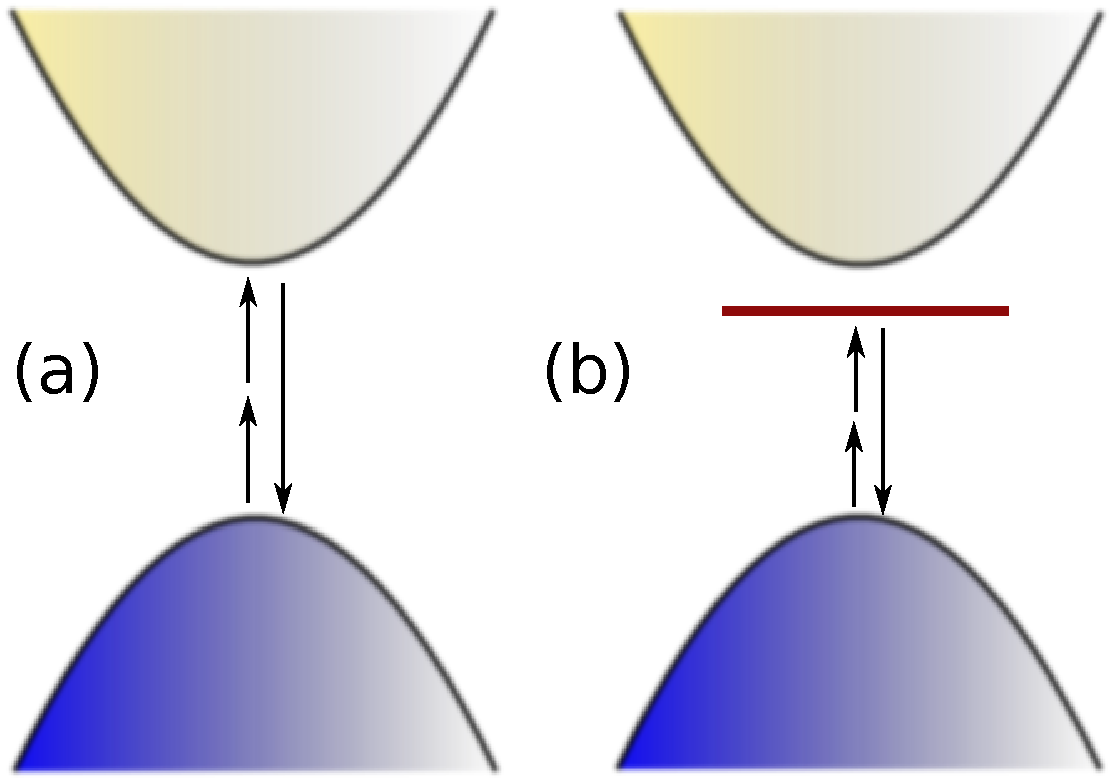
\includegraphics[width=0.4\textwidth]{Figures/exciton}
\caption{\footnotesize{Schematic representation of  (a) the SHG within the IPA, or (b) accounting for electron-hole interaction. In (a) SHG is given simply by transitions between the valence (blue) and conduction (yellow) manifolds; in (b) electron-hole may lead to the formation of a bound exciton, an atomic-like level (dark red) into the fundamental band gap that strongly modifies the SHG. \label{schemeshg}}}  
\end{center}
\end{wrapfigure}   

On a more fundamental level, SHG is extremely interesting since it allows to probe symmetries and excitations not visible in the linear regime\cite{doi:10.1021/nl401561r,kumar2013second}.   In both cases it is %it may be 
important to have the support and guide from the theory through accurate and reliable numerical simulations.



Using the methodology developed in the previous chapters we investigate the SHG in h-BN and MoS$_2$ monolayers, two materials with promising applications in optoelectronic and photonic devices. These two materials share an hexagonal 2D structure but their electronic and optical properties are quite different. The optical absorption of h-BN is dominated by two very bright and strongly bound excitons.\cite{PhysRevLett.96.126104,PhysRevLett.100.189701} Instead the optical absorption of MoS$_2$ is characterised by a weakly bound exciton, split by spin-orbit coupling,\cite{PhysRevLett.105.136805} and by a brighter exciton in the continuum at about 3~eV.\cite{molina2013effect} 

The interpretation of the linear optical properties of these materials has been possible through \emph{ab initio} calculations (e.g. Refs.~\cite{molina2013effect,PhysRevLett.100.189701}). These computational studies captured the peculiar nature of excitons in nanostructures\cite{scholes2006excitons} by the inclusion of the relevant correlation effects.
%In particular state-of-the-art calculations employ the combination of the Bethe-Salpeter equation\cite{strinati} in static ladder approximation with the $GW$ quasiparticle corrections\cite{Aulbur1996,noteGW} on the band structure (BSE+$GW$) that accurately and efficiently describes the electron-hole interaction\cite{strinati}---the fundamental process in exciton formation. 


In contrast, large part of calculations of nonlinear optical properties employ the independent particle approximation\cite{guo2005second,margulis2013optical} (IPA) which are inadequate for low dimensional systems (see Fig.~\ref{schemeshg}).\cite{scholes2006excitons} 
%From a theoretical point of view, calculations of the optical response beyond the linear regime still remain a challenge.
%Different approaches have been proposed to include effects beyond the IPA. 
%Local field effects have been included\cite{PhysRevB.34.3700} to take into account crystal inhomogeneities, but only few works tackled the problem of correlation. 
%In fact, the approaches developed within response theory to study neutral excitations in the linear regime, such as Many-Body perturbation theory or Time-dependent Density Functional Theory (TDDFT), become extremely involved when applied to the non-linear response.\cite{Leitsmann2005,PhysRevA.83.062122,PhysRevB.61.8341,Adolph1998,Chang2002,PhysRevB.80.165318,PhysRevB.82.235201} Within Many-body perturbation theory the diagrams that enter in the calculation of the second and third order susceptibilities, 
%$\chi^{(2)}$ and $\chi^{(3)}$, 
%are so intricate that their implementation becomes awkward if not impracticable (see for instance Fig.~3 of Ref.~\cite{PhysRevB.80.165318}). Even within the ``simpler'' TDDFT, equations for the second order optical response has been solved only for particular approximations of the exchange-correlation functional,\cite{PhysRevB.82.235201} or have been limited to the static response.\cite{kirtman:1294}

%On the other hand, correlation effects can easily be included into real-time approaches, in which the response functions are obtained from the time propagation of ``simpler'' objects as the single particle Green's function, the density matrix or the density.\cite{takimoto:154114}
%However these approaches have been often limited to finite systems, such as atoms, molecules or clusters, since the calculation of the bulk polarization in solids poses additional challenges: when imposing periodic boundary conditions (PBC) the full polarization cannot be expressed in term of an Hermitian operator but it is related to the variation of the Berry's phase.\cite{KSV1}

%In the chapters we combined Modern Theory of Polarization\cite{RevModPhys.66.899} with Time-dependent Bethe-Salpeter(TD-BSE)\cite{strinati} into an \emph{ab-initio} approach to calculate non-linear response in solids beyond the IPA. In particular in the linear response limit this approach corresponds to the BSE+$GW$,\cite{attaccalite} so successful for optical properties of low dimensional materials (see Chapters~\ref{chapterberry} and \ref{chaptercorr}). 
In order to investigate the contribution of correlation effects on the SHG spectra of h-BN and MoS$_2$ monolayers, we use the TD-BSE approach developed in this chapter. For both materials we disclose the signature of bound excitons and show that excitonic effects not only significantly modify the shape of the spectrum with respect to the IPA, but strongly enhance its intensity. In the conclusions we comment how this finding may open the possibility of engineering the SHG signal in these materials. 

%For the MoS$_2$ layer we used the experimental lattice constant of the bulk MoS$_2$ as in Ref.~\cite{molina2013effect} and an inter-layer distance of 30 a.u. The electron-ion term was approximated using norm conserving pseudo-potentials and exchange correlation term using the Perdew, Burke and Ernzerhof functional [Phys. Rev. Lett. 77, 3865 (1996)]. The $GW$ correction of $0.72~eV$  was taken from Ref.~\cite{molina2013effect}. The screened Coulomb interaction was calculated using 100 bands and a cutoff of 2 Ha on the dielectric matrix dimensions. SHG was obtained using a $21\times21\times1$ k-point grid, 18 bands within IPA and TDH, and bands between the 3$^\text{rd}$ and the 16$\text{th}$ for the TDSHF.


%Calculations of the Kohn-Sham band structure for the zero-field systems are performed with the pseudopotential planewave code {\sc Abinit},~\cite{abinit} while SHG spectra are calculated using a develop version of the{\sc Yambo} code,~\cite{yambo} where Eqs.~\eqref{tdbse_shf}-\eqref{berryP} have been implemented.
%Working with a planewave basis set, we simulate isolated monolayers by a slab supercell approach with large inter-sheet distance. 
%Eq.~\eqref{tdbse_shf} is numerical integrated with a time-step of $\Delta t = 0.0025$~fs, that guarantees accuracy and stable results. In order to reproduce experimental conditions we use a laser intensity of $I = 500~$kW/cm$^2$, we add a dephasing term with $\tau=6$~fs in Eq.~\ref{tdbse_shf} to simulate a finite broadening of about $0.2~eV$,\cite{nloptics2013} and propagate Eq.~\eqref{tdbse_shf} for $55$~fs for each laser frequency.



\subsubsection{Results}
In order to simulate isolated hexagonal-BN and MSo$_2$ monolayers we used a supercell approach with a large distance between the sheets. Then we propagate the time-dependent Schr\"odinger equation with the Hamiltonian derived in Eq.~\ref{mbhamiltonian}. Non-linear coefficients are obtained from the real-time polarisation [Eq~\ref{berryP2} ] as described in chapter~\ref{chapterberry} and all numerical details are presented in Ref.~\cite{PhysRevB.89.081102}. 

\subsubsection{h-BN monolayer}
%As illustrated in the previous section we obtained the second harmonic response from the time propagation of the Eq.~\eqref{tdbse_shf}.  By excluding or including the different terms in the right side of this equation we can  investigate their effect on the second harmonic response. We start our discussion from the h-BN sheet. 
Hexagonal Boron-Nitride is a transparent insulating material with a large band gap of about $6~eV$. Its optical properties are dominated by strong bound excitons and they are nearly independent from the layers arrangement.\cite{PhysRevLett.96.126104,PhysRevLett.100.189701} The single layer h-BN inherits all these properties from its bulk counterpart.
\begin{figure}[H]
    \vspace{-0.32cm}
    \centering
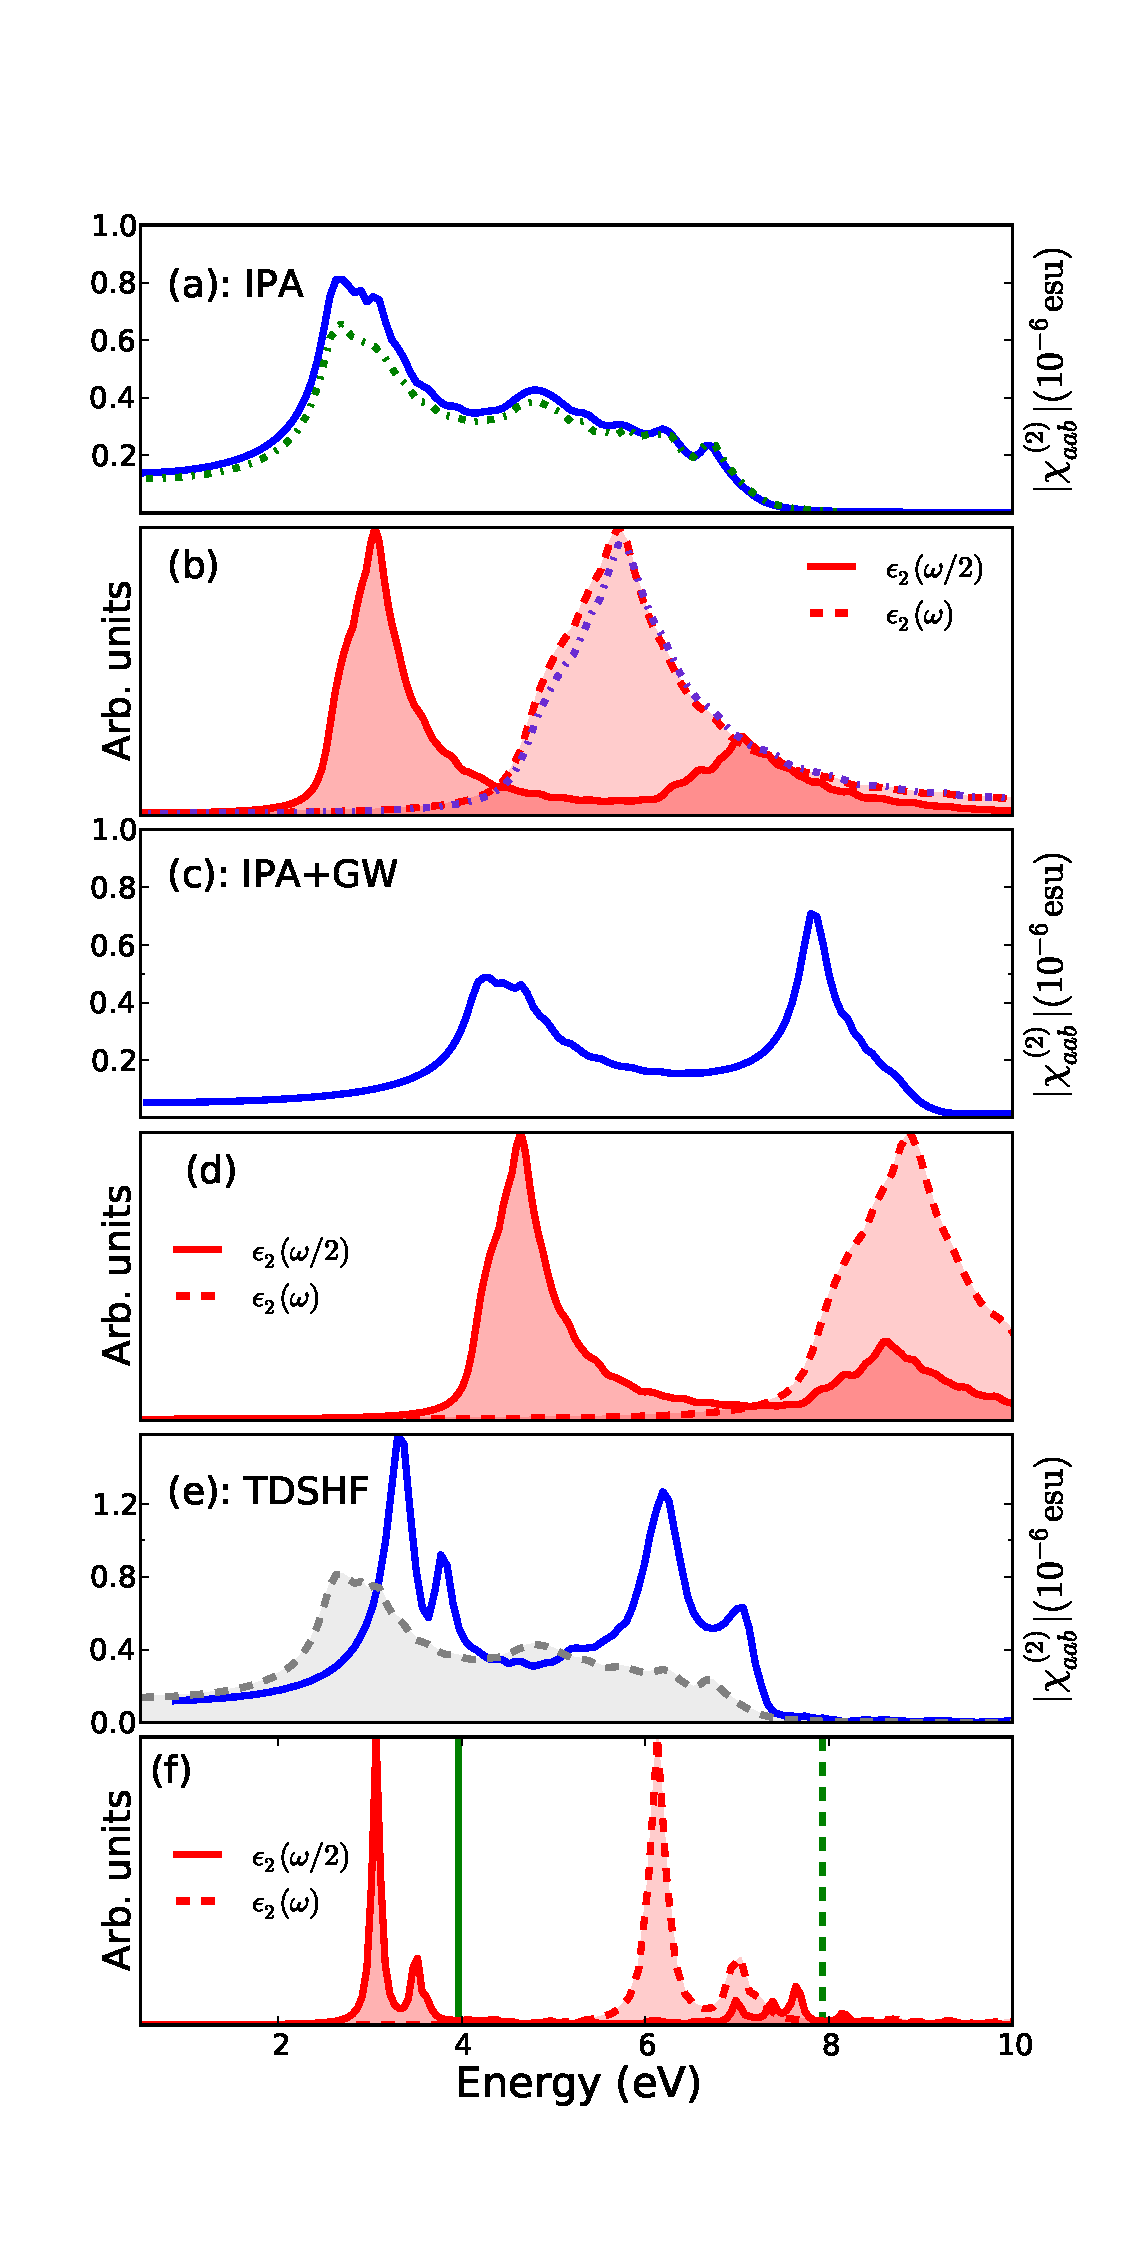
\includegraphics[width=0.5\textwidth]{Figures/eps_and_X2}
    \vspace{-0.85cm}
\caption{\footnotesize{SHG spectra for the h-BN monolayer at different levels of theory [Eq.~\eqref{mbhamiltonian}]: (a) IPA (blue continuous line) and TDH (green dashed line); (c) IPA + GW correction (blue continuous line); (e) TD-BSE (blue continuous line) and IPA (grey dashed line). The imaginary part of the dielectric constant at both $\omega/2$ (red continuous line) and $\omega$ (red dashed line) is reported in (b), (d) and (f) for IPA, TDH and TD-BSE respectively. (f) also reports the LRC spectrum (blue dotted-dashed line) whose intensity has been reduced by a factor 0.5 for presentation reasons. The vertical lines represent the $GW$ fundamental gap (green dashed line) and half of the $GW$ fundamental gap (green continuous line). \label{absX2bn} [Figure from Ref.\cite{PhysRevB.89.081102}]}}
\end{figure}


\begin{figure}[h]
\centering
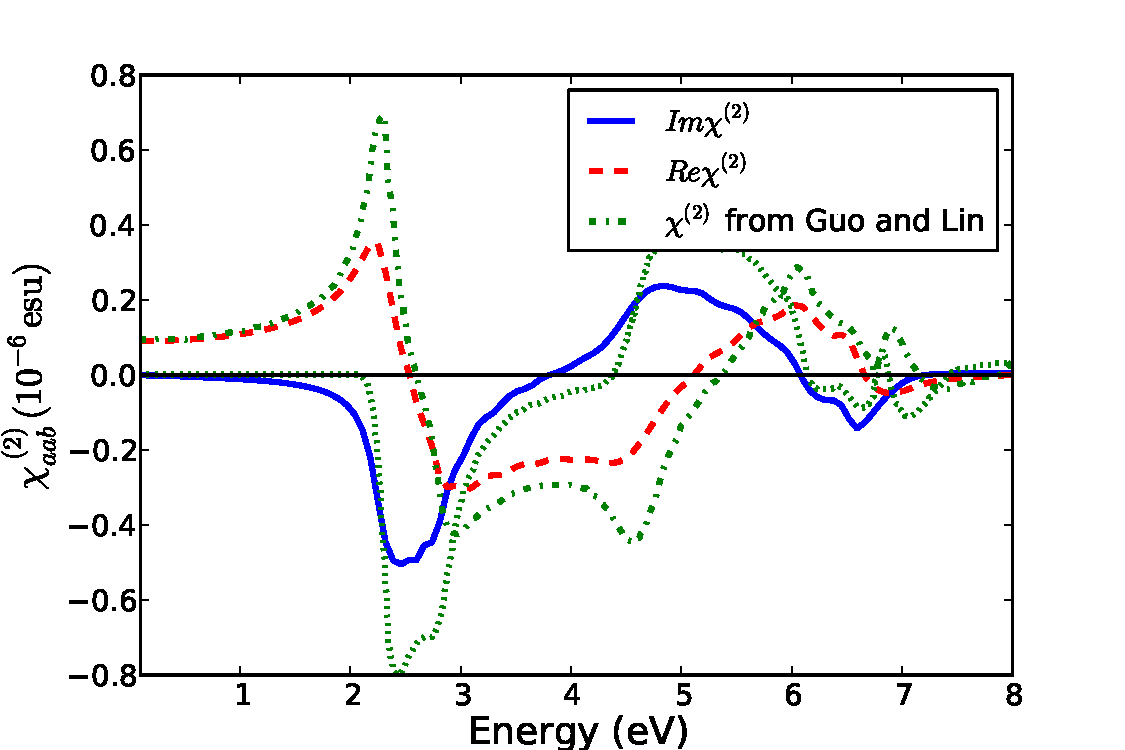
\includegraphics[width=0.6\textwidth]{Figures/IPX2}
\caption{\footnotesize{SHG for the h-BN monolayer within the IPA: the real (red dashed line) and the imaginary (blue continuous line) part of the calculated $\chi^{(2)}_{aab}$ are compared with the real (green dashed-dotted line) and imaginary part (green dotted line) of the $\chitwo$ obtained by Guo and Lin.\cite{guo2005second}[Figure from Ref.\cite{PhysRevB.89.081102}]}\label{X2bn}}
\end{figure}
In Fig.~\ref{absX2bn} we report the calculated absolute value of $\chi^{(2)}_{aab} (\omega)$ at different levels of approximation. $\chi^{(2)}_{aab} (\omega)$, where $a$ and $b$ are the in-plane Cartesian directions, is the only independent in-plane component of $\chi^{(2)} (\omega)$: all other components can be obtained from the $\chi^{(2)}_{aab} (\omega)$ with simple symmetry considerations, for instance $\chi^{(2)}_{bbb} (\omega)=-\chi^{(2)}_{aab} (\omega)$. 

At IPA level [Fig.~\ref{absX2bn}(a)], the SHG presents a peak at $2.3~eV$ and a broad structure between $4 - 7 eV$. By comparison with the imaginary part of the dielectric constant $\epsilon_2$ both at $\omega/2$ and  $\omega$ [Fig.~\ref{absX2bn}(b)] calculated at the same level of theory, we can attribute the peak at $2.3~eV$ to two-photon resonances with $\pi \to \pi^*$ transitions, and the broad structure mostly to one-photon resonances with $\pi \to \pi^*$ transitions, with contributions around $7 eV$ of two-photon resonances with $\sigma \to \sigma^*$ transitions.

 


This level of theory is the one usually employed in theoretical calculations of SHG: in fact results for the h-BN monolayer were previously obtained by Guo and Lin:~\cite{guo2005second} Fig.~\ref{X2bn} shows a very good agreement between our results and those obtained in Ref.~\cite{guo2005second}. In the following we show how effects beyond the IPA---that is the additional terms in Eq.~\eqref{mbhamiltonian}---modify the SHG spectrum.        


\begin{figure}[h]
\centering
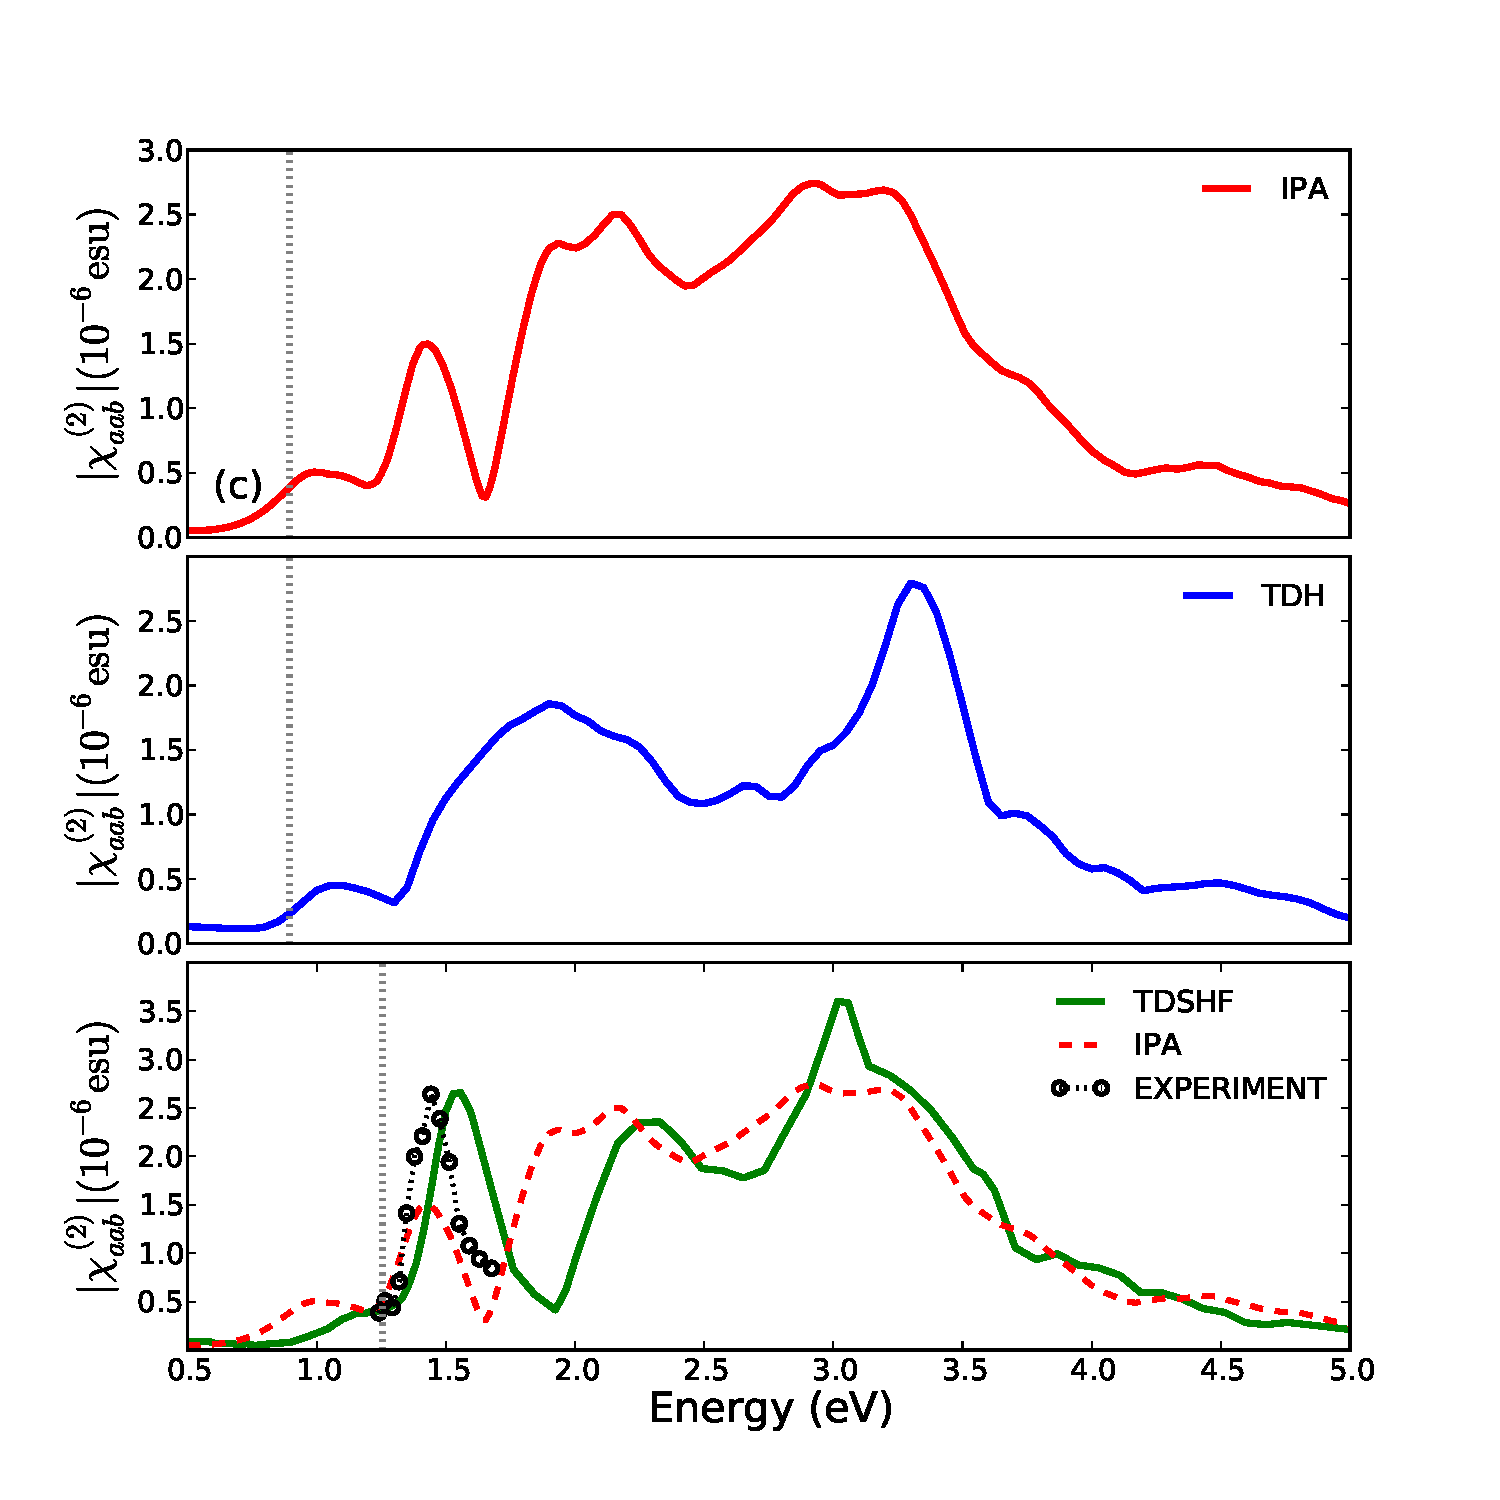
\includegraphics[width=.7\textwidth]{Figures/absX2MoS2}
\caption{\footnotesize{SHG in the MoS$_2$ monolayer at different levels of the theory [Eq.~\eqref{mbhamiltonian}]: (a) IPA (red squares), (b) TDH (blue circles) and (c) TD-BSE (green squares). The latter is compared with IPA (red dashed line) and experimental results of Malard et al.\cite{PhysRevB.87.201401} (black circles). Since the experimental SHG is measured relatively to the substrate, we renormalized the experimental spectrum to match the intensity of the $~ 1.5 eV$ peak in the calculated spectrum. The grey dotted vertical lines indicate the energy of half of the Kohn-Sham band gap in (a) and (b), and of  half of the $GW$ band gap in (c).[Figure from Ref.\cite{PhysRevB.89.081102}] }\label{fg:SHMoS2}}
\end{figure} 


We start by adding crystal local field effects, included at the TDH level [Fig.~\ref{absX2bn}(a)]. Because of the weak in-plane inhomogeneity of the h-BN, local field effects are quite small---though they are not negligible as for the absorption spectrum  [Fig.~\ref{absX2bn}(b)]---and results in the reduction of about 20\% of the peak at $2.3~eV$. Next we consider the renormalization of the band structure by quasiparticle corrections within the $GW$ approximation (IPA+$GW$) [Fig.~\ref{absX2bn}(c)]. For h-BN this renormalization can be safely approximated by a rigid shift of the conduction bands. Differently from the absorption spectrum [Fig.~\ref{absX2bn}(d)], the SHG is not simply shifted by $GW$ corrections, but its shape changes remarkably as a consequence of the more involved poles structure of the second order susceptibility.~\cite{PhysRevB.82.235201,hughes1996calculation}
In fact, the IPA+$GW$ shows two peaks: the first at about $4~eV$ is the shifted two-photon $\pi \to \pi^*$  resonances peak which is attenuated by 40\% with respect to IPA  [Fig.~\ref{absX2bn} (a)]; the second very pronounced peak at about $8~eV$ comes from the interference of  $\pi \to \pi^*$  one-photon resonances and  $\sigma \to \sigma^*$ two-photon resonances.  

Finally, in Fig.~\ref{absX2bn}(e) we consider the full Hamiltonian in Eq.~\eqref{mbhamiltonian}. In particular we add the self-energy terms that introduces an attractive interaction between the excited electrons and holes\cite{strinati}. The SHG spectrum presents four sharp and strong peaks and its onset is red-shifted by about $1~eV$ with respect to the the IPA+$GW$ [Fig.~\ref{absX2bn} (c)]. By comparing with the imaginary part of the dielectric constant $\epsilon_2$ both at $\omega/2$ and  $\omega$ [Fig.~\ref{absX2bn} (f)] calculated at the same level of theory, the two couples of peaks can be identified respectively as the two- and one-photon resonances with the excitons at $6$ and $7~eV$.  Fig.~\ref{absX2bn}(e) also shows again the SHG within the IPA to emphasise the striking difference between the two spectra: the TD-BSE spectrum presents features that are missing in IPA and more importantly is twice as strong than IPA at the exciton resonances. 

%Excitonic peaks are well visible, well below the band gap, in the optical spectra (see panel $d)$ of Fig.~\ref{absX2bn}). They are responsible for the high efficient luminescence in h-BN crystals.\cite{watanabe} Here we show that excitonic effects appear also in the second order response. Resonances with the first bound exciton gives rise to the first peak in the second harmonic (Fig.~\ref{absX2bn} panels $c)$ and $d)$). Moreover also the second exciton is clearly visible in the SHG because resonances with this exciton are the cause of the second peak in $|\chi^{(2)}|$. The electron-hole interaction not only change the position of the peaks in the SHG but strongly enhanced their intensity. At the resonance the first peak is two times stronger than the IPA case. This
%is one of the main finding of this paper, that resonances
%between bound excitons can enhanced the SHG signal in
%low dimensional materials, as we demonstrated for the h-BN.


\begin{center}
\begin{table}[h]
\small
\begin{tabular}{c|cc|c|c|c}
\hline
$|\chi^{(2)}_{aab} (0)| $ (pm/V) & \multicolumn{2}{c|}{IPA} & TDH & IPA+G$_0$W$_0$ & TD-BSE  \\
\hline
 h-BN &  57.1(3)  & [40.7] & 48.5(5) &  21.8(1)  & 46.9(2)  \\
%\hline
%MoS$_2$  &  &     &               &     &   \\
\hline
\end{tabular}
\caption{$\omega\rightarrow 0$ limit of $\chi^{(2)}_{aab} (-2\omega,\omega,\omega)$ of the h-BN monolayer at different levels of the theory [Eq.~\eqref{mbhamiltonian}]. As a comparison, for the IPA we report in square brackets also the value obtained in Ref.~\cite{guo2005second}.\label{tab1}}  
\end{table}
\end{center} 

In  Table~\ref{tab1} we report  the value of the second optical susceptibility at $\omega=0$, $\chi^{(2)}(\omega \to 0)$, extrapolated from the SHG  behaviour at small frequencies.    
Again, at the IPA level our result agrees with the one of Guo and Lin\cite{guo2005second} within the error bar. Adding the effects beyond IPA, modifies the $\chi^{(2)}(\omega \to 0)$ value, and in particular within TD-BSE we found a value smaller by about 10\% than at the IPA level.

Excitonic effects in SHG spectrum have been treated as well in a TD-DFT framework\cite{PhysRevB.82.235201} by using the so-called long-range-corrected (LRC) approximation,\cite{LRC} a semi-empirical simple model for the screened electron-hole attraction, that includes only the long-range part of the interaction. In Fig.~\ref{absX2bn}(f) we see the $\epsilon_2$ calculated within the LRC approximation: as earlier recognised, this approximation fails for strong excitons. In fact by tuning the empirical parameter for the screening we could get the position of the first exciton, though its intensity is strongly overestimated (see caption of Fig.~\ref{absX2bn}), but in no way we could get the second excitonic peak. Those pitfalls would be reflected in the SHG spectrum, though we did not test it in our approach. Then clearly the h-BN monolayer and similar low dimensional materials with strong excitonic effects cannot be treated within the approach proposed in Ref.~\cite{PhysRevB.82.235201}.

\subsubsection{MoS$_2$ monolayer}
MoS$_2$ differs from h-BN in several aspects. First, while the h-BN has an indirect minimum band gap as its bulk counterpart, in MoS$_2$ an indirect-to-direct band gap transition occurs passing from the bulk to the monolayer due to the vanishing interlayer interaction.  Second, spin-orbit coupling plays an important role in this material, splitting the top valence bands, as visible from the absorption spectrum, presenting a double peak at the onset.\cite{PhysRevLett.105.136805} Third, Mo and S atoms in the MoS$_2$ monolayer are on different planes resulting in a larger inhomogeneity than for the h-BN.
Figure~\ref{fg:SHMoS2} presents the SHG spectra $|\chi^{(2)}_{aab}|$  at the different level of approximations of Eq.~\eqref{mbhamiltonian}. At the lowest IPA level [Fig.~\ref{fg:SHMoS2} (a)], the SHG presents three main features: a small peak at 1~eV, which originates from two-photon resonances with transitions close to the minimum gap at the $K$ point; a larger peak around $1.5$~eV, which originates from two-photon resonances with transitions along the high symmetry axis between $\Gamma$ and $K$ where the highest valence and lowest conduction bands are flat and there is a high density of states; a broad structure between $2-3.5$~eV which originates from one-photon resonances with transitions at $K$ and along $\Gamma-K$ and two-photon resonances with transitions to higher conduction bands. Note that we do not include spin-orbit coupling in Eq.~\eqref{mbhamiltonian}. 
The latter is expected to split the lowest peak into two weaker sub-peaks~\cite{molina2013effect}, but to leave unaffected the second peak, the most important when it comes to applications and central to our analysis.\cite{PhysRevB.87.201401}  
Because of the quite strong inhomogeneity of the MoS$_2$ monolayer, the addition of crystal local field effects within the TDH strongly modifies the SHG  [Fig.~\ref{fg:SHMoS2} (b)]. 
In particular the main peak at $1.5$~eV merges with the plateau at $2$~eV while a peak appears around $3.3$~eV.
%Could be added, but refs are needed: local fields affects transitions between $\Gamma$ and $K$ that involve both Mo d and S p, while transitions at K, atomic-like, localized on Mo, not affected 
Finally, within the TD-BSE, we add the quasi-particle effects and electron-hole interaction  [Fig.~\ref{fg:SHMoS2} (c)]. The small shoulder around $1$~eV, below half of the $GW$ gap (1.25 eV, grey dotted vertical line in the figure), originates from two-photon resonances with the bound excitons around $2$~eV which are well visible in the experimental absorption spectra.\cite{PhysRevLett.105.136805}  The main peak at about $1.5$~eV, present in the IPA spectrum but washed out by local field effects within the TDH, is restored by the electron-hole interaction and its intensity is two times larger than in the IPA case. This peak corresponds to a two-photon resonance with the bright exciton at 3~eV observed in the absorption spectrum,\cite{molina2013effect} and its position and shape agrees well with the experimental measurements of Malard et al.\cite{PhysRevB.87.201401} for the SHG between $1.2-1.7$~eV, also reported in Fig.~\ref{fg:SHMoS2}(c). The calculated spectrum also shows a strong one-photon resonance with this exciton at 3~eV.
With respect to h-BN, where the IPA is clearly inadequate when compared with the TD-BSE [Fig.~\ref{absX2bn}(e)], here IPA and TD-BSE  presents similar features, at approximately the same position [Fig.~\ref{fg:SHMoS2} (c)]. In fact, this different behaviour could be expected from the linear optical response of these materials, as discussed in the Introduction. Nevertheless, also in this case the electron-hole interaction proved to be key for SHG as it doubles the intensity of the main peak in the visible range, the one that is relevant for applications in nonlinear optics.      
\section{Conclusions}
We presented a novel approach for  \emph{ab-initio} calculation of linear and non-linear
optical properties in bulk materials and nano-structures that uses a
time-dependent extension of the BSE.
The proposed approach combines the flexibility of a real-time approach
with the strength of MBPT in capturing electron-correlation.  It
allows to perform computationally feasible simulations beyond the
linear regime.
Being the approach based on the non-equilibrium Green's Function theory, it is possible to
include effects such as lifetimes, electron-electron
scattering\cite{bsedynamic} and electron-phonon
coupling\cite{giustino2016electron} in a systematic way.
We validated the TD-BSE in the case of {\it h}-BN calculating
the optical absorption and comparing it with the results from equilibrium
GW+BSE, then we applied the same methodology to study the non-linear response of two-dimensional
crystals.
We found that electron-hole interaction greatly enhances the SHG signal in 2D crystals with respect to the independent-particle picture. Specifically, for the h-BN monolayer one- and two-photons resonances with bound excitons produce strong signatures in the SHG spectrum with intensities two times larger than expected from the IPA. In MoS$_2$, though the shape of the spectrum is not strikingly modified by excitonic effects as for h-BN, the electron-hole interaction enhances, again by about 200\%, the SHG signal in the visible range with respect to the IPA. 
This finding may provide a spin-off for the quest of materials with high SHG. In fact---given that the SHG signal depends largely on the electron-hole interaction that in turn depends on the electronic screening---the SHG intensity can be tuned by changing the electronic screening. Then, it may be possible, as proposed in Ref.~\cite{gao2012artificially}, to engineer meta-materials with a high SHG by combining layers of different 2D crystals\cite{gao2012artificially} so to change the electronic screening, and further enhance the electron-hole interaction effects.
As side finding, our results emphasise that it is critical for theoretical and computational approaches to accurately include electron-hole interaction, together with quasiparticle and local field effects, in order to predict non-linear optical response in low dimensional materials. In this regard, our recently proposed approach~\cite{nloptics2013,attaccalite} is quite promising as it imports into the very flexible real-time framework---apt to treat nonlinear optics---the combination of BSE+$GW$ successfully applied to the linear optical response of low-dimensional materials.\\ 
The interested reader can find other applications of the TD-BSE in Refs.~\cite{attaccalite2015strong,attaccalite1d}.
